\documentclass{article}
% I just added all the things, if you have problems build, try deleting the
% naggin packages, fat chance I don't even use it.
\usepackage{amsmath}
\usepackage{txfonts}
\usepackage{booktabs}
\usepackage{color}
\usepackage{bussproofs}
\usepackage{graphicx}
\usepackage{pifont}
\usepackage{qtree}
\usepackage{tikz}
\usepackage{amssymb}
\usetikzlibrary{automata,arrows,positioning,calc}
\usepackage{listings}
\usepackage{hyperref}
\newenvironment{scprooftree}[1]%
{\gdef\scalefactor{#1}\begin{center}\proofSkipAmount \leavevmode}%
{\scalebox{\scalefactor}{\DisplayProof}\proofSkipAmount \end{center} }

\newcommand{\brcell}[2][l]{%
	\begin{tabular}[#1]{@{}l@{}}#2\end{tabular}}

\begin{document}
\lstset{language=Java}
\author{Jappie Klooster}
\title{Logic, Kripke and Chaos}
\maketitle

\section{Introduction}
This will be an introduction to modal logic coming from someone who followed
` hbo informatica' as pre study.

In here I will write down the things I think are important for understanding
modal logic and how to proof things in that system.

% Before starting I just want to lay out the idea here, everytime I hear
% kripke, I imagine someone waving his arm and shouting KRIPKE in anger.
% Not that anyone will ever read these comments but its a funny idea.

This course was thought by John-Jules Meyer. The `theoretic' part focused
on the ideas behind the logics, while the `practical' focussed on writing
propper proofs. I guess I'll treat both in here.

There are 2 main sources of information I'll use, the slides by John Jules
and the modal logic paper for artificial intelligence by rosja mastop to help
me with the practical part. 
% In truth I didn't understand much of the practicals, just giving a bunch
% of examples is not a good way of teaching how to write proofs.
% This paper seems to explain it in a more structural way.

\section{Basic modal logic}
Express intensional (context/situation-sensitve) notations such as: 
Knowledge, Belief, Obligation, Action and Time.

\subsection{Modal langauge}

Imports all the things from propositional logic and is extended
with the modal operators ($\Box\phi,\Diamond\phi$) which can be read as:

\begin{tabular}{ll}
	Symbol & Definition \\ \toprule
	$\Box\phi$ & It is \emph{necesarry} that $\phi$ \\
	$\Diamond\phi$ & it is \emph{possible} that $\phi$

\end{tabular}

\noindent
Also $\neg\Box\neg\phi = \Diamond\phi$ and
$\neg\Diamond\neg\phi = \Box\phi$. So you could theoratically
drop one to create the other.
% where $\phi$ is an object I guess?

\paragraph{Semantics} Kripke %KRIPKE, *waves arm*.
model/frame $M=\langle S,\pi,R \rangle$

\begin{tabular}{ll}
	Symbol & Definition \\ \toprule
	% worlds implies mutability, states, well a state is by definition 
	% imutable. I'm pretty sure we want immutability in these kind 
	% off logics
	$S$ & Is a set of \emph{states (or worlds)} \\
	$\pi$ & Is a truth assignment function $\pi : S \times AT \to {tt, ff}$ \\
	$R$	& $R \subseteq S \times S$ is an \emph{accesibility relation}\\
\end{tabular}

\subsection{Interpertation}

\begin{center}
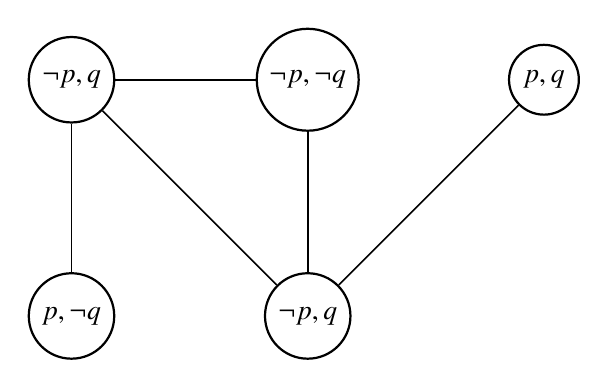
\begin{tikzpicture}[auto, >=stealth', auto, semithick, node distance=3cm]
\tikzstyle{every state}=[fill=white,draw=black,thick,text=black,scale=1]
\node[state]    (S)            {$\neg p, q$};
\node[state]    (A)[below of=S]{$p, \neg q$};
\node[state]    (B)[right of=S]{$\neg p, \neg q$};
\node[state]    (C)[right of=B]{$p, q$};
\node[state]    (E)[below of=B]{$\neg p, q$};
\path
(S)   edge[above]     		(A)
(S)   edge[above]     		(E)
(S)   edge[above]     		(B)
(B)    edge[above]     		(E)
(E)    edge[above]     		(C);
\end{tikzpicture}
\end{center}

Like classical propositional logic, but now realtive to a model and a state:

\[ M,s \vDash \phi \]

thus:

\begin{tabular}{lll}
	Modal & $\Leftrightarrow$ & Interpertation \\ \toprule
$M,s \vDash p$ & $\Leftrightarrow$ & $\pi(s,p) = tt$ \\
$M,s \vDash \phi \wedge \varphi $ & $\Leftrightarrow$ & $ M,s \vDash \phi
\mbox{ and }M,s\vDash \varphi$ \\
$M,s \vDash \Box \phi $ & $\Leftrightarrow$ & $ M,t \vDash \phi $ for 
\emph{every} $t$ such that $R(s,t)$ \\
$M,s \vDash \Diamond \phi $ & $\Leftrightarrow$ & $ M,t \vDash \phi $ for 
\emph{some} $t$ such that $R(s,t)$ \\\bottomrule
\end{tabular}

\subsection{Validity}
\begin{tabular}{llll}
	Definition & Denotation & $\Leftrightarrow$ & Interpertation \\ \toprule

$\phi$ is \emph{valid} in a model $M= \langle S, \pi, R \rangle$ &
$M\vDash\phi$ & $\Leftrightarrow$ & $M,s \vDash \phi$ for all $s \in S$ \\

$\phi$ is \emph{valid}  &
$\vDash\phi$ & $\Leftrightarrow$ & $M\vDash\phi$ for all Kripke models $M$ \\

$\phi$ is \emph{valid} wrt class $\zeta$ &
$\zeta\vDash\phi$ & $\Leftrightarrow$ & $M\vDash\phi$ for all Kripke models
$M \in \zeta$ \\\bottomrule
\end{tabular}

The last one doesn't occur often.

\section{System K}
We try to  axiomatize validities.

\paragraph{Axioms} We import all (or enough) propositional tautologies.
The K axiom ($(\Box\phi \wedge \Box (\phi \to \varphi))\to\Box\varphi$) is added.

\paragraph{Rules} Modes ponens
\begin{prooftree}
	\AxiomC{$\phi$}
	\AxiomC{$\phi \to \varphi$}
	\BinaryInfC{$\varphi$}
\end{prooftree}

Necisitation rule:
\begin{prooftree}
	\AxiomC{$\phi$}
	\UnaryInfC{$\Box\phi$}
\end{prooftree}

\subparagraph{Caution} the necisitation is different from the invalid
assertion: $\phi \to \Box \phi$.

\subsection{Derivability in K}
A \emph{derivation} of a formula $\phi$ is a finite sequence of formulas
$\phi_1, \dots \phi_n = \phi$. where each $\phi_i$ for $1 \ge i \ge n$
is either an instance of the acioms (or rather axiom schemes), or the
conclusion of one of the rules of which the premises have
been derived already, i.e{.} appear as $\phi_j$ in the sequance with
$j < i$.

% sad thing is I understand this crap now.
When we can derive an epistemic formula $\phi$ by using the axioms
and rules of $K_{(m)}$ we write $K_{(m)} \vdash \phi$

System $K_{(m)}$ is \emph{sound and complete}. This means
that exactly ll valid modal assertions can be obtained by derivations in
system $K_{(m)}$.

\[\vDash \phi \Leftrightarrow K_{(m)} \vdash \phi\]

% I leave out the (non) theoroms, it seems overkill.

\section{Dynamic logic}
An example of an (indexed) version of system $K$ is dynamic logic,
wehre the $\Box$ modality is associated with the execution results of
a program / action.

$\Box_\alpha$, normally written $[\alpha]$ 
with reading $[\alpha]\phi$: after exuction of $\alpha$ it holds that $\phi$

\[<\alpha>\phi = \neg [\alpha] \neg \phi \]

\subsection{Semantics}
Accessibility relation $R_\alpha$ for every action $\alpha$

\begin{tabular}{llll}
	% I added the natural collumn, because otherwise I won't remember.
	% Translating something in a different notation is stupid.
	notation & = & definition & natural \\ \toprule
	$R_{\alpha;\beta}$ & = & $R_\alpha \circ R_\beta$ &
	execute from $R_\alpha$ until including $R_\beta$\\
	$R_{\alpha+\beta}$ & = & $R_\alpha \cup R_\beta$ &
	execute $R_\alpha$ or $R_\beta$\\
	$R_{\alpha*}$ & = & $R_\alpha*$ &
	Execute an arbitrary times \\ \bottomrule
\end{tabular}

\subsection{Interpertation}
\begin{tabular}{lll}
	Modal & $\Leftrightarrow$ & Interpertation \\ \toprule
	$M,s \vDash [\alpha]\phi$ & $\Leftrightarrow$ &
	for all $s'$ with $R_\alpha(s,s'): M,s' \vDash \phi$ \\
	$M,s \vDash <\alpha>\phi$ & $\Leftrightarrow$ &
	for some $s'$ with $R_\alpha(s,s'): M,s' \vDash \phi$ \\\bottomrule
\end{tabular}

\section{Special properties of accessibility relations}
\begin{tabular}{lll}
	R is \dots& if\dots & natural language \\ \toprule
	reflexive & $\forall s \in S(s,s) \in R$ & all s are linked with 
	themselves\\

	transitive & $\forall s,t,u \in S:(s,t) \in R \& (t,u) \in R \Rightarrow
	(s,u) \in R$ & \brcell{if s is related to t, and t is related to u,  \\
		then s has a relation with u, \\ in other words, you can make shortcuts}\\

	symmetrical &$\forall s,t \in S:(s,t) \in R \Rightarrow (t,s) \in R$ &
	undirected, can go back and forth\\
	euclidiean & $\forall s,t,u \in S:(s,t) \in R \& (s,u) \in R \Rightarrow
	(t,u) \in R$ & \brcell{if s has a relation with t and u, then u and t \\
	have a relation to, you can make triangles.} \\
	serial & $\forall s \in S \exists t \in S (s,t) \in R$&
	\brcell{All states in S are connected to \\ at least one other state in S}\\
	an equivalance relation& R is \emph{reflexive, transitive and 
	symetrical}& \brcell{the states R links to have something in \\ 
	common (not equal?)} \\ \bottomrule
\end{tabular}
\end{document}
